\begin{figure}[b!]
\centering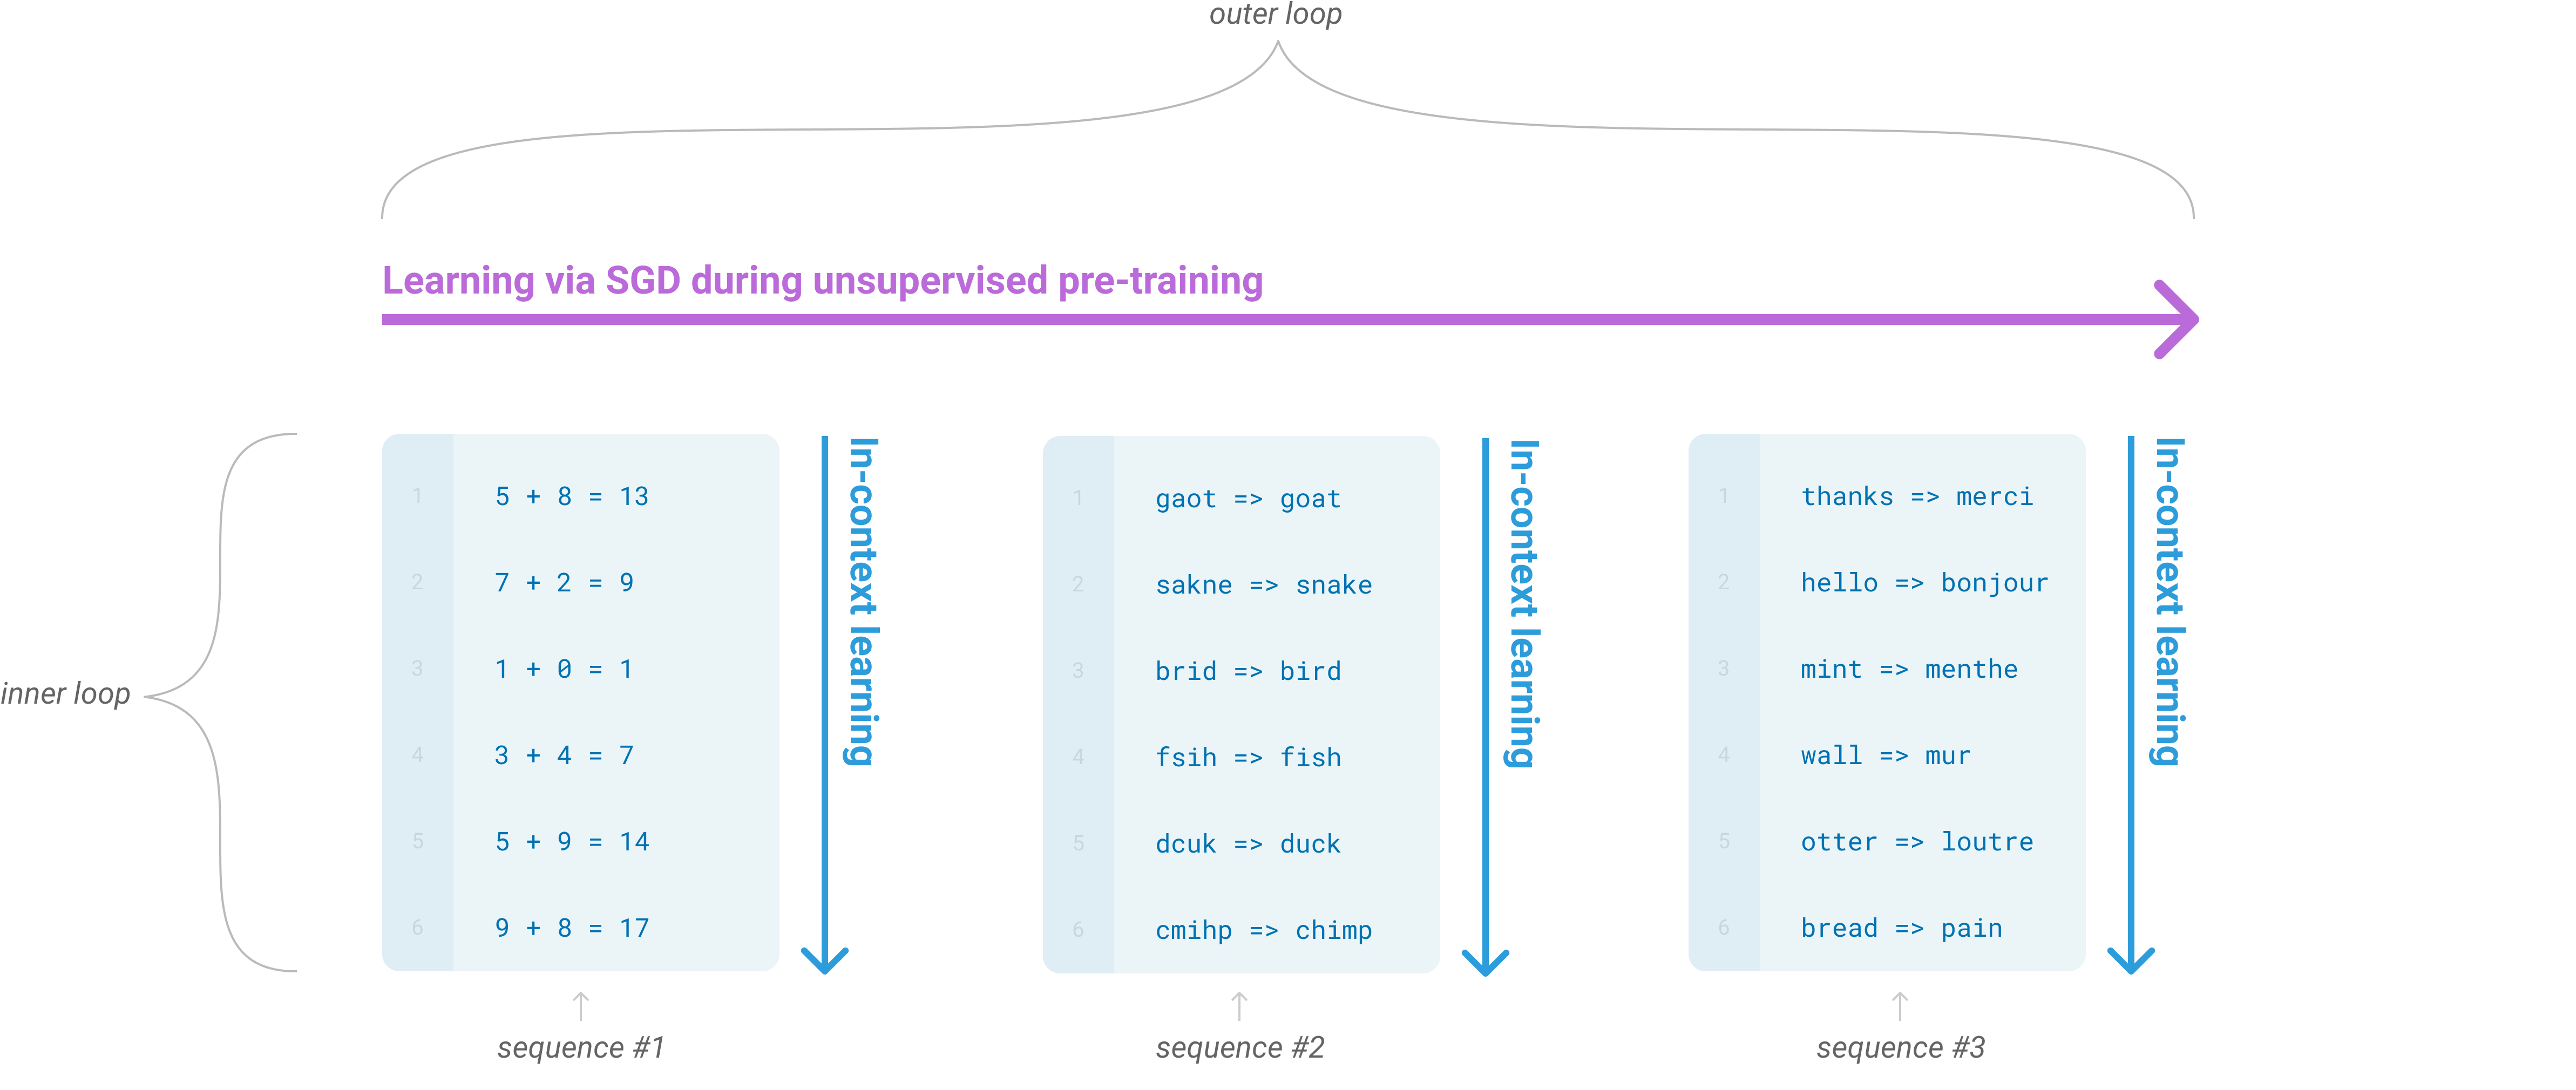
\includegraphics[width=1.0\linewidth]{figures/metalearning.png}
\caption{\textbf{Language model meta-learning.} During unsupervised pre-training, a language model develops a broad set of skills and pattern recognition abilities. It then uses these abilities at inference time to rapidly adapt to or recognize the desired task. We use the term ``in-context learning" to describe the inner loop of this process, which occurs within the forward-pass upon each sequence. The sequences in this diagram are not intended to be representative of the data a model would see during pre-training, but are intended to show that there are sometimes repeated sub-tasks embedded within a single sequence.
}
\label{figure:metalearning}
\end{figure}